%-------------------------------------------------------------------------------------------------
%
%  Skeleton for bachelor and master thesis reports at the Software Lab
%-----------------------------------------------------------------------------------------
%
% USAGE:      compile with PDFLaTeX
%
% HISTORY:    - written by Sascha A. Stoeter <stoeter@iris.ethz.ch>, www.stoeter.com, 02.06.2004
%             - modified by Martin Probst, 18.08.2004
%             - extended and adapted for use at LST by Oliver Trachsel, 2007-08-21
%             - modified for use at Software Lab by Michael Pradel, Nov 2014
%             - modified for use at U Stuttgart by Michael Pradel, Sep 2020
%-------------------------------------------------------------------------------------------------
\documentclass[11pt,a4paper]{book}
\usepackage{solareport}

% -------------------------------------------------------------------------------------------------
% Add needed packages. Some generally useful packages are listed for
% your convenience.
% -------------------------------------------------------------------------------------------------
\usepackage{subfigure}                          % enable the use of subfigures
\usepackage[thickspace,thinqspace]{SIunits}     %
\usepackage[plainpages=false,pdfpagelabels]{hyperref}    % enable hyperlinks in pdf/ps Docs
\usepackage{listings}                           % to embed source code

% -------------------------------------------------------------------------------------------------
% Select type of thesis
% -------------------------------------------------------------------------------------------------
%\def\thesistype{Bachelor}
\def\thesistype{Master}

% -------------------------------------------------------------------------------------------------
% Set names
% -------------------------------------------------------------------------------------------------
\def\thesisauthor{Piyush Krishan Bajaj}
\def\thesisadvisor{Islem Bouzenia} % leave empty if directly advised by Michael Pradel
\def\studyprogram{INFOTECH} % e.g., Computer Science or INFOTECH

% -------------------------------------------------------------------------------------------------
% Set dates
% -------------------------------------------------------------------------------------------------
\def\thesisstartdate{November 7, 2022} 
\def\thesisenddate{May 7, 2023} 


% -------------------------------------------------------------------------------------------------
% Beginning of the main document body
% -------------------------------------------------------------------------------------------------
\begin{document}

% -------------------------------------------------------------------------------------------------
% Front matter with title page, table of contents, and abstracts 
% -------------------------------------------------------------------------------------------------
\frontmatter

% Title page: set title
\thesistitlepage{DyPyBench: A Benchmark of Executable Python Software}

% Abstract must not be longer than one page per language. English and
% German abstracts are mandatory.
\chapter*{Abstract}
Short summary of thesis.

\chapter*{Zusammenfassung}
Kurzfassung der Arbeit.

% Table of contents
\tableofcontents

% -------------------------------------------------------------------------------------------------
% Main document body
% -------------------------------------------------------------------------------------------------
\mainmatter
\chapter{Introduction}
\label{s:Introduction}
Python is a popular interpreted, high-level and general-purpose programming language that is easy to read and has a concise syntax, making it suitable for novice and experienced programmers. It supports various programming paradigms and uses dynamic typing and efficient memory management techniques. Python is also highly extensible through the use of modules, making it a preferred choice for adding programmable interfaces to existing applications \cite{Python_language_wiki}. Python provides dynamic features such as dynamic typing, dynamic object creation, dynamic attribute access, dynamic module loading and dynamic function definition.

Python is a popular language for analysis, bug detection, performance checking, and vulnerability testing due to its easy-to-learn syntax, large community, and extensive libraries. Its strong support for data analysis, visualization, and statistical analysis, as well as cross-platform compatibility, make it an excellent choice for developing cross-platform software and tools. Python also has a range of testing and debugging tools, including built-in frameworks like unittest and pytest, and third-party tools like PyCharm and PyDev. These tools help developers detect and fix bugs and improve code performance.

Java, C++ and Python are commonly used high-level programming languages, which are powerful, object-oriented and have dynamic features which make them ideal for complex applications in software development. The dynamic features of Java include automatic memory management, garbage collection, reflections and exceptions, whereas C++ provides the dynamic features such as templates, dynamic memory allocation and runtime dynamic linking. In order to evaluate these dynamic features of a language, a dynamic benchmark can be used, which involves measuring the performance of a system or application while it is running under real-world conditions.  Unlike static benchmarks, which test a system or application under controlled conditions, dynamic benchmarks attempt to simulate the actual usage patterns of users and applications in order to measure performance more accurately. Java and C++, both have a number of such dynamic benchmarks available such as Java Microbenchmark Harness (JMH) \cite{JMH}, The DeCapo Benchmark \cite{DaCapo_2006}, The Computer Language Benchmarks Game \cite{C++_Benchmark1} and Boost.Benchmarks \cite{Boost_Benchmarks}. Although, Python has some dynamic benchmarks available such as PyPerformance \cite{PyPerformance} and Apache Bench \cite{Apache_Benchmark}, these are not general purpose benchmarks like those provided for Java and C++. These python benchmarks measure the performance of the programs for a single dynamic feature in a specific domain under the real-world conditions.

A general-purpose dynamic benchmark of python programs would help us to analyze different dynamic features of the language such as those mentioned above in real world conditions. And at the same time, it would also encapsulated a wide range of application domains which are brought to the table because of the popularity and wide spread usage of python for building complex applications including machine learning, web development, server development and virtual environments to name a few.  Such a benchmark can be used with existing tools such as systrace \cite{systrace} to run and evaluate the diverse python programs, and at the same time allow new tools such as DynaPyt \cite{DynaPyt2022} to perform the required analysis. This general-purpose benchmark can also be used to generate a dataset for machine learning (ML) and deep learning (DL) tasks of software engineering such as bug detection \cite{DeepBugs2018}, code completion \cite{code_completion}, quality analysis \cite{Code_analysis_1, Code_analysis_2}, code refactoring \cite{code_refactoring}, and testing \cite{testing_1, testing_2, testing_3}. Such ML and DL tasks have the potential to improve the productivity, efficiency and quality of code. However, the accuracy and effectiveness of these tasks depend on the quality and quantity of the data used to train the model.

The past decade has seen tremendous progress in the field of artificial intelligence thanks to the resurgence of neural networks through deep learning. This has helped improve the ability for computers to see, hear, and understand the world around them, leading to dramatic advances in the application of AI to many fields of science and other areas of human endeavor \cite{Machine_Learning_decade}. Machine learning, which is a branch of artificial intelligence (AI) and computer science focuses on the use of data and algorithms to imitate the way that humans learn, gradually improving its accuracy. Over the last couple of decades, the technological advances in storage and processing power have enabled some innovative products based on machine learning, such as Netflix’s recommendation engine and self-driving cars \cite{Machine_Learning}.

Tasks such as bug detection \cite{DeepBugs2018}, code completion \cite{code_completion}, quality analysis \cite{Code_analysis_1, Code_analysis_2}, code refactoring \cite{code_refactoring}, and testing \cite{testing_1, testing_2, testing_3} can be performed using machine learning algorithms by analysing software source code and improving the development process. Such program analysis has the potential to improve the productivity, efficiency and quality of code. Machine learning works by training algorithms on data to make predictions or take actions based on that data. There are three main steps in the machine learning process namely, Data collection and preparation, model training, and finally Model evaluation and deployment. Data collection is a critical step as the quality and quantity of the data used to train a model can greatly impact its accuracy and effectiveness. When collecting data for machine learning in software development, it's important to focus on the right kind of data to train the algorithm on. This data should be relevant, diverse, and representative of the problem being solved. For example, if a machine learning model is being trained to detect bugs in code, the data should consist of code snippets with bugs as well as code snippets without bugs.

The program analysis algorithms of machine learning, either use the code snippets which are available via the source code\cite{static_code_analysis} or logs which are generated by the execution of the software \cite{loglens}. In both of these cases we do not get the detailed information related to the run time behaviour of the executed software. Run time behaviour can provide us a different perspective and has the potential to provide deeper insights which can help us in improving the code and the development process. For example, ***

As described above, DynaPyt is a framework which provides us the insights into the run time behaviour of python programs. Since we are already seeing the usefulness of machine learning in the software engineering tasks, we can combine the best of both of these to achieve a program analysis tool which uses machine learning to improve development process of code using the run time behaviour of python programs. At the time of writing this thesis, there are no framework or benchmark tools available which combine them. With this thesis we provide a framework,  which is a benchmark of executable python software which can be used to generate data set for machine learning tasks in software engineering tasks such as code generation, test case generation etc. for researchers and developers. 

The benchmark consists of 50 executable python software from diverse application domains which Python covers being a highly popular general purpose programming language. By using the DynaPyt framework, the data set generated is able to encapsulate the run time behaviour of python programs. In DyPyBench framework, we provide three different program analysis tasks of software engineering using machine learning approach. The first task *** . The second task ***. Finally, the third task ***. In this thesis, we have further used the machine learning algorithm ** to test and evaluate our framework. The results are ***. 


\chapter{Background and Motivation}
\label{s:Background}
In this chapter, we provide an overview of the topics needed to understand the work done in this thesis.

\section{Benchmarks}
Benchmarks are tools used to measure the performance and efficiency of computer systems or components.
They evaluate the speed and quality of hardware, software, and applications to optimize performance, identify bottlenecks, and make informed decisions about system configurations.
There are many types of benchmarks that measure specific aspects of a computer system, such as processing power, memory speed, disk access time, or application performance.
Benchmarks simulate real-world workloads and produce scores that can be compared across different systems or components.
% However, benchmark results may not always be reliable due to factors such as hardware compatibility, software optimization, and testing conditions.
To ensure accuracy and reliability, it is important to use multiple benchmarks, perform tests under different conditions, and interpret results carefully.
Overall, benchmarks are an essential tool for evaluating computer systems and components, enabling users to optimize performance and make informed decisions about hardware and software configurations.

\section{Docker}
Docker is a platform that enables developers to containerize an application and its dependencies, making it easier to deploy and manage software across different environments.
Docker containers are lightweight and portable, and Docker Hub is a cloud-based repository where developers can store and share their Docker containers.
It provides a centralized platform for managing container images and features such as image management, automated builds, and security scanning, which help developers maintain the quality and security of their containers.
Docker Hub also includes a registry service, which simplifies the deployment process and makes it easier to manage and scale applications in different environments.
In summary, Docker and Docker Hub are powerful tools that enable developers to build, deploy, and manage software more efficiently and effectively through containerization and centralized repository management.

\section{Scripting in Software Development}
Scripting in software development refers to the use of scripting languages to automate various tasks, such as building and deploying software, managing databases, and testing software.
Scripting is a way to execute a sequence of commands automatically, without the need for manual intervention.
By using scripts, developers can save time and effort, and focus on other important tasks. Python and Bash are popular scripting languages used in software development.
Python is known for its readability and ease of use across different operating systems.
Bash is a Unix shell scripting language used primarily in Linux and Unix operating systems, and is powerful for system administration and automation.
% Scripting enables developers and administrators to automate repetitive tasks and improve efficiency.

\section{Code Analysis Frameworks}
Code analysis frameworks are tools used in software development to analyze source code and identify potential issues, vulnerabilities, and errors.
They help developers to maintain code quality, improve security, and ensure compliance with coding standards and best practices.
% These frameworks identify issues such as code smells, potential security vulnerabilities, coding errors, and violations of coding standards.
Popular code analysis frameworks include SonarQube, Checkstyle, ESLint, and Fortify, among others.
These frameworks are valuable tools for software developers as they provide detailed reporting and analysis features, enforce coding standards, identify potential errors, and help to remediate security vulnerabilities.
Ultimately, code analysis frameworks help developers to write better, more secure, and higher-quality software code.

\section{DynaPyt}
DynaPyt is a tool for dynamic analysis of Python code.
It aims to provide insights into the behavior of Python programs, such as performance and memory usage, by analyzing the runtime behavior of code.
DynaPyt provides several features, such as the ability to collect data on function calls, memory allocation, and object creation, and to visualize the results in a user-friendly interface.
The tool is designed to be easy to use and to work with existing Python code, making it accessible to a wide range of users, from researchers to developers.
The tool makes it possible to get a detailed understanding of the behavior of Python programs.
This information can be used to identify performance bottlenecks and optimize the program for better performance.
With its ease of use, flexibility, and range of features, DynaPyt is a valuable tool for anyone working with Python code.

\section{Neural Models for Code Analysis}
Neural models or neural networks can be used in code analysis to improve the accuracy and efficiency of code analysis tasks.
These models can be trained to classify code, generate code, and detect code smells, potential security vulnerabilities, coding errors, and violations of coding standards.
By analyzing patterns and relationships within code, neural models can identify potential issues that may not be easily detected through manual code analysis.
Neural models have the potential to provide developers with new tools for maintaining code quality, improving security, and ensuring compliance with coding standards and best practices.

\section{Call Graphs}
Call graphs are visual representations of the relationships between functions or methods in a program used in software development.
They help developers understand the flow of control in a program, identify potential bottlenecks, optimize performance, and debug issues more quickly.
Call graphs can be created manually or automatically using static and dynamic analysis techniques.
Tools such as Eclipse Call Graph, Doxygen, and Graphviz provide different levels of detail and customization options for call graphs.
In summary, call graphs are an essential tool for understanding and analyzing complex software systems, helping developers to visualize the relationships between functions and optimize code for better performance and maintainability.

\chapter{Methodology}
\label{s:Methodology}
In this chapter, we describe the approach which we have adopted to create the dynamic benchmark of executable Python software.
The overall workflow of the approach is shown in the Figure \ref{fig:overall_approach}.

\begin{figure}[ht]
\centering
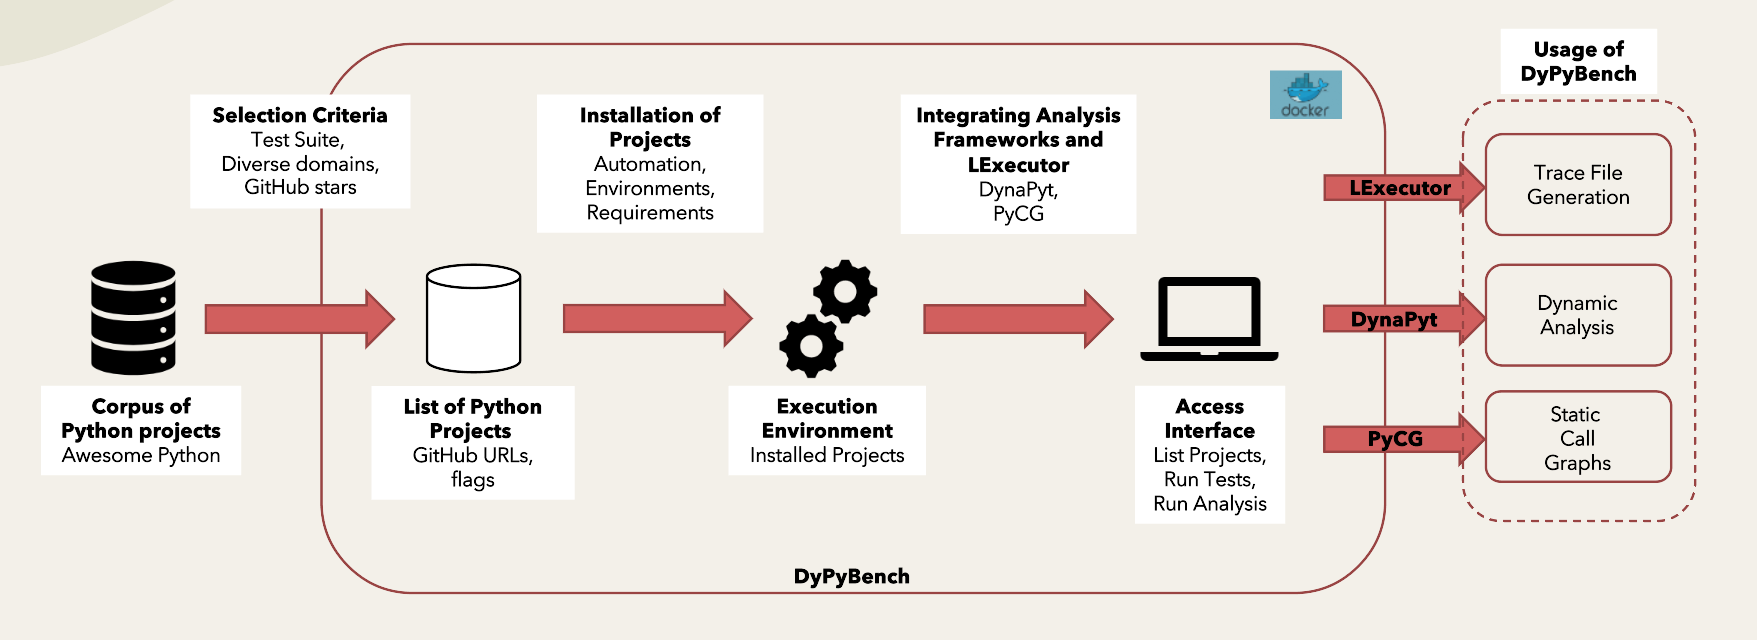
\includegraphics[width=1\linewidth]{figures/approach/DyPyBench3.png}
\caption[Approach]{\label{fig:overall_approach}Overall Approach of DyPyBench.}
\end{figure}

As can be seen from the Figure \ref{fig:overall_approach}, we first apply the selection criteria to the corpus of Python projects to select a number of projects (Section \ref{approach:project selection}) to generate a list.
The list of projects is then used to prepare the benchmark by installing the projects and their dependencies using automation (Section \ref{approach:benchmark preparation}).
We proceed by integrating the two analysis frameworks, DynaPyt and PyCG (Section \ref{approach:analysis framework}). 
We also integrate LExecutor into the benchmark (Section \ref{approach:LExecutor}).
Finally, we package and export the benchmark with an access interface for use by researchers and developers (Section \ref{approach:artifact packaging and interface}).   

With the provided approach, we aim to achieve the properties as listed below.
\begin{itemize}
    \item \textbf{Large-scale} The benchmark should comprise tens of real-world open-source projects, allowing users to evaluate their analyses on a wide range of code.
    \item \textbf{Diverse} The benchmark should contain projects from a diverse range of application domains that reflect the state of today's Python ecosystem.
    \item \textbf{Ready-to-run} There should be a single interface to run each project in the benchmark, making it easy for users to set up and execute the entire benchmark.
    \item \textbf{Ready-to-analyze} To enable dynamic analyses, the executions of all projects in the benchmark should be set up to be analyzed.
    \item \textbf{Compositional} To help users understand the behavior of specific projects or even individual test cases, it should be easy to run subsets of full benchmark.
    \item \textbf{Long-term} The benchmark should be built using commonly used tools and formats, e.g., pip and Docker, to ensure its longevity.
    \item \textbf{Extensibility} The benchmark should be easily extensible, allowing users to add, remove or update the tools, frameworks and projects.  
\end{itemize}

\section{Projects Selection}
\label{approach:project selection}
In this section, first we discuss about the available Python projects and why we use awesome-python as a corpus for our benchmark (Section \ref{approach:corpus of python projects}).
Then we discuss about the three selection criteria which we use to select projects from the corpus to make our benchmark diverse and large-scale (Section \ref{approach:selection criteria}).
\subsection{Corpus of Python Projects}
\label{approach:corpus of python projects}
Python's ease of use and popularity, as well as the usage in different domains has led to a large number of projects being developed and made available to the community as open-source projects.
GitHub alone contains a lot of open-source repositories that have Python as their primary programming language.
Furthermore, there are some GitHub repositories which provide a collection of Python projects such as Awesome Python \footnote{https://github.com/vinta/awesome-python/}, Awesome Python Applications \footnote{https://github.com/mahmoud/awesome-python-applications} and Python Projects \footnote{https://github.com/practical-tutorials/project-based-learning}.
These collections of projects also provide us with a classification for the projects based on the application domains.
In this work, we use the awesome-python project which contains a curated list of some of the awesome open-source Python projects including libraries, frameworks and software. 
The awesome-python project is the corpus of projects for our benchmark as it contains a collection of 679 Python projects.
Awesome-python further classifies these projects into 92 main categories, out of which some of the categories are further divided into sub-categories.
These sub-categories contain the subset of the main category based on technology, tool and their intended usage.
For example, the sub-categories for Distributed Computing are Batch Processing and Stream Processing which are the two intended ways of processing data.
The top ten categories and the number of projects in those are listed in Table \ref{table:awesome-python}.
Appendix \ref{appendix:tables} provides more details on the various categories and number of projects in each category provided by awesome-python project.

\begin{table}[ht]
    \centering
    \begin{tabular}{lc}
    \hline
    \textbf{Category} & \textbf{Number of Projects}\\
    \hline
    Testing & 30\\
    Text Processing & 22\\
    Science & 21\\
    Code analysis & 18\\
    Debugging Tools & 18\\
    Specific Formats Processing & 18\\
    Command Line Tools & 17\\
    GUI development & 16\\
    Database Drivers & 15\\
    Image Processing & 15\\
    Others (82) & 483\\
    \hline
    \end{tabular}
    \caption{Top Ten Project Categories (Awesome Python).}
    \label{table:awesome-python}
\end{table}

\subsection{Selection Criteria}
\label{approach:selection criteria}
To select projects for our benchmark, we use three criteria namely diverse domain, test suite execution with pytest and GitHub stars.
To ensure the diversity property presented before, we sample the projects from across multiple categories covering as many application domains as possible provided by the awesome-python corpus.
Since, the suggested approach creates a dynamic benchmark we focus on the projects for which we can perform execution.
Test suites provide us with files that can easily execute the code using testing libraries such as pytest and unittest.
Thus we select projects with test suites which can run using the popular pytest library that is also compatible with unittest. 
Lastly, to ensure the criterion of GitHub stars, we select projects which have at least 500 stars on its GitHub repository. 
The number of stars a project has on GitHub is an indication of how popular and well-regarded it is in the community.
More stars generally mean more people have found the project useful and it has a larger user base and community of contributors \cite{github_stars}.
We find 500 stars to be sufficient since it allows us to have the required number of well-regarded projects.  

\section{Benchmark Preparation}
\label{approach:benchmark preparation}
In this section, we start with a discussion about how we use flags in a list of projects to automate the installation process (Section \ref{approach:list of projects}).
We then discuss about how we use these flags in our work to install 50 projects (Section \ref{approach:bash scripts}).
Finally, we discuss about the working environment which is created by the installation of the above 50 projects (Section \ref{approach:collection of projects}).

\subsection{Collecting and Structuring a List of Projects}
\label{approach:list of projects}
Applying the selection criteria as described before, we select 50 open-source Python projects.
Although, the installation and setup of these projects follow similar steps, there are certain differences which vary from project to project.
For example, the path and the name of requirements file to install dependencies varies for each project.
Some of these differences can be attributed to the directory structure of source code present in the GitHub repository.
The Figure \ref{fig:setup} shows the installation steps for two sample Python projects.
The blue colored text indicates similarities, whereas the red colored text indicates the differences.
\begin{figure}[ht]
    \centering
    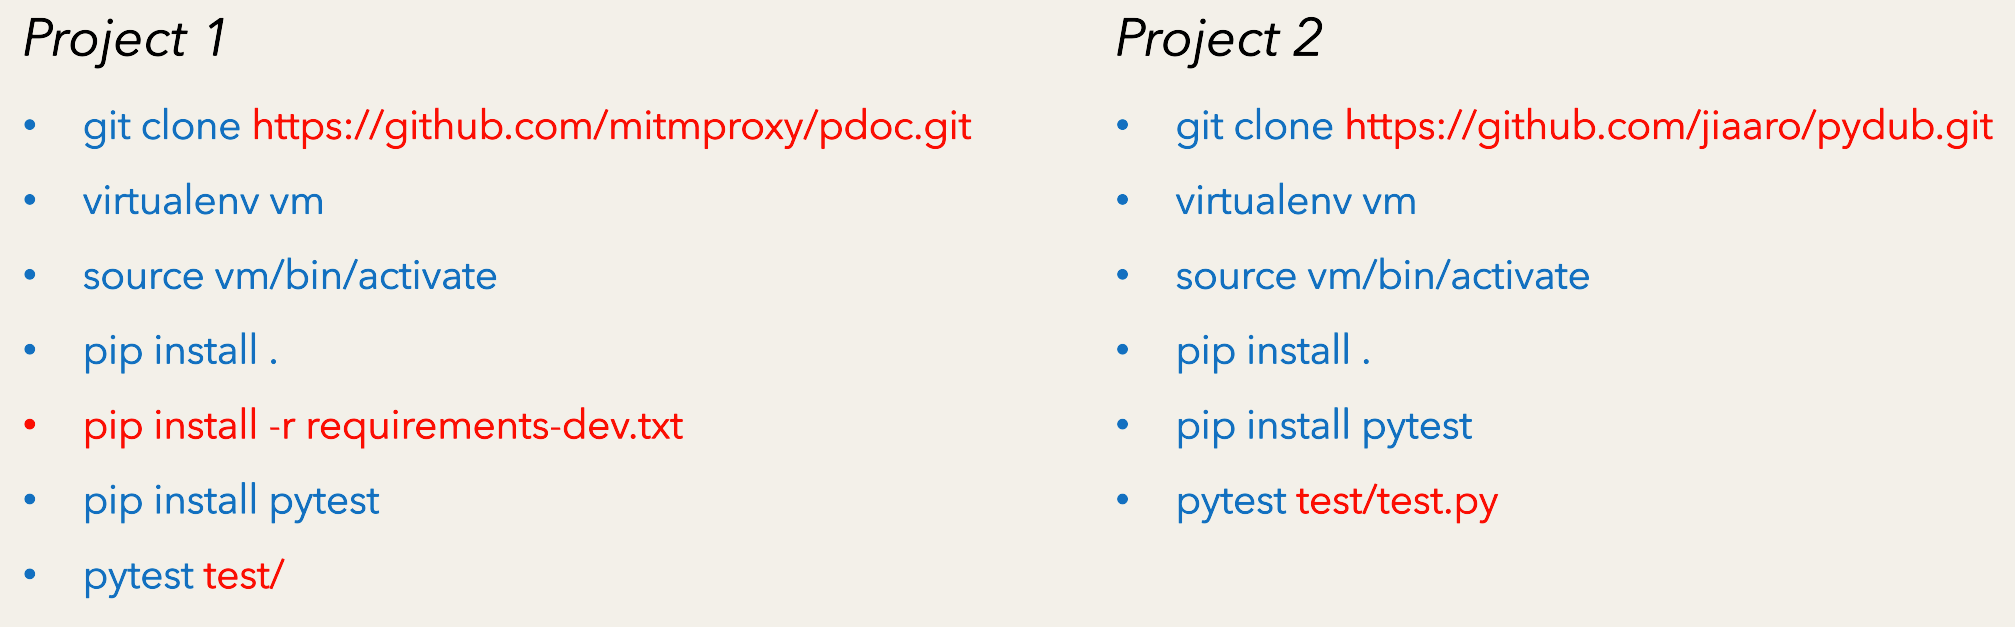
\includegraphics[width=1\linewidth]{figures/approach/Setup-differences.png}
    \caption{Installation and Execution of Projects (Similarities and Differences).}
    \label{fig:setup}
\end{figure}

In order to automate the process of installation and setup of projects, we need a way to work around these differences for each project.
In this approach, we use a list with specific flags inside a text file to handle the aforementioned differences.
This structure of a single entry  which represents one project in this list is $ \textbf{project\_url requirement\_flag *requirement\_file test\_suite} $.
In the structure, \textit{project\_url} corresponds to Git URL for the project, whereas \textit{requirement\_flag} represents the information pertaining to the presence or absence of requirement file.
The \textit{requirement\_flag} can have 2 possible values, \textit{rt} and \textit{t}.
The next flag in the entry is the \textit{requirement\_file}, which is the path of requirement file. 
This flag is optional and is present only when the \textit{requirement\_flag} is \textit{rt}.
The final flag in the entry is \textit{test\_suite} that contains the path of the test directory which is needed to execute tests.
Furthermore, it is easy to add, modify or delete an entry from the text file which makes the benchmark extensible.
Table \ref{table:list of projects} shows two example entries in the list.
The first entry is a project with a requirement file present at src/requirements.txt and test suite in the directory tests, while the second entry does not contain a requirement file and its test suite is present in the directory src/tests.

\begin{table}[ht]
    \centering
    \begin{tabular}{llll}
    % \hline
    % \textbf{GitHub URL} & \textbf{Flag} & \textbf{Requirement File} & \textbf{Test Path}\\
    \hline
    https://github.com/test/test-project.git & rt & src/requirement.txt & tests\\
    https://github.com/tester/test-project.git & t & src/tests\\
    \hline
    \end{tabular}
    \caption{List of Projects (Collection Text File Structure).}
    \label{table:list of projects}
\end{table}

\subsection{Installation of Projects}
\label{approach:bash scripts}
The above list of projects with the specified flags in a text file is used to automatically install the projects with a single command.
With the URL to the GitHub Repository and optional requirement file, we perform a series of steps to install each project with its required dependencies.
Firstly, we clone the repository from the URL provided in the text file to get the source code.
We then create a virtual environment to avoid dependency conflicts between different projects.
Then we install the project to the virtual environment using the source code cloned before. 
Finally, if there is a requirement file we install the dependencies specified in this file to the virtual environment.
The mundane and repetitive task of performing these steps for each of the 50 projects is automated using scripts.
Scripts can handle repetition through the use of loops such as for and while.
They can also work with exceptional cases using conditionals such as if else statements.  

\subsection{Execution Environment}
\label{approach:collection of projects}
The automated installation of projects provide us with a collection of 50 Python projects.
This collection forms the pool of projects which our benchmark provides to perform code analysis or to generate training data for neural models.
Each project installed using the automation is present inside a sub-folder in the collection.
This makes it easier to work on individual projects when needed.
When a particular project from the collection needs to used, a duplicate copy of the same is created.
This ensures the long-term usage of the projects in the benchmark by preserving the projects and their virtual environments.
The dynamic nature of Python and open-source ecosystems results in frequent changes to the projects.
Another advantage provided by duplication is avoiding the re-installation of projects which saves significant time and effort. 

\section{Integrating Analysis Frameworks}
\label{approach:analysis framework}
To satisfy the property of ready-to-analyze, we need to integrate some code analysis frameworks into our benchmark.
In our project, we incorporate two such frameworks, namely, DynaPyt,  which a general purpose dynamic analysis framework and PyCG, which is a static analysis framework to generate call graphs.
The following sections explain the integration of these two frameworks.
\subsection{DynaPyt}
In this work, we use DynaPyt to perform dynamic analysis for generating call graphs.
But it is possible to perform any dynamic analysis using DynaPyt.
We first develop the Call Graph Analysis using the function pre\_call hook provided by DynaPyt.
This is then used to instrument the source code of the project.
Finally, the test suite of the instrumented project is executed which generates a run-time call graph.
The steps of instrumentation and execution of tests is integrated into the access interface. 

\subsection{PyCG}
In this work, we use PyCG to generate call graphs for the collection of projects.
The test files are provided as the entry point for generating the the call graphs.
The required arguments and command to generate the call graphs based on static code analysis is integrated into the access interface.

\section{Integrating LExecutor}
\label{approach:LExecutor}
While code analysis provides a usage scenario of our benchmark, we add another usage scenario of collecting data for fine-tuning a neural model.
This is done using LExecutor, which provides a command to fine-tune the model and improve its accuracy using the training data.
In our approach, we first instrument the project which we need to add into the training data.
We then run the test suite of the instrumented project, which generates one or more trace files.
These trace files are then fed to the LExecutor which provides a command to use the trace files and generate training data.
The instrumentation and test suite execution are integrated into the access interface provided by the benchmark.

\section{Artifact Packaging and Interface}
\label{approach:artifact packaging and interface}
In this section, we first provide the details regarding the access interface we design to provide make the benchmark easily accessible (Section \ref{approach:access interface}).
Then we talk about why we use Docker to package and export our benchmark and how it makes the benchmark extensible (Section \ref{approach:packing and exporting}).

\subsection{Access Interface}
\label{approach:access interface}
To provide an easy access to the projects and the analysis frameworks in the benchmark, we create a single command line access interface.
Along with easy access, we also aim to make the benchmark ready-to-run and ready-to-analyze with this interface. 
The access interface provides various alternatives to the end user specified by the command line options.
The available options are provided in the Table \ref{table:access interface options}, where the first column specifies the option and the second column provides description of its usage.
With the options \textit{dynapyt\_instrument}, \textit{dynapyt\_run}, \textit{lex\_instrument}, \textit{lex\_test} and \textit{pycg}, one can specify a variable number of projects which makes the benchmark highly versatile.

\begin{table}[ht]
    \centering
    \begin{tabular}{ll}
    \hline
    \textbf{Option} & \textbf{Description}\\
    \hline
    list    & List the project number, name and GitHub URL\\
    test    & Run test suite of specified projects\\
    save    & Save standard output and error to file specified\\
    timeout & Timeout in seconds for commands\\
    update\_dynapyt\_source   & Clone or update source code of DynaPyt\\
    update\_lex\_source   & Clone or update source code of LExecutor\\
    dynapyt\_instrument  & Instrument files for DynaPyt\\
    dynapyt\_file    & Specify file to use for instrumentation of DynaPyt\\
    dynapyt\_analysis    & Specify the analysis to perform for DynaPyt\\
    dynapyt\_run & Execute DynaPyt analysis for specified projects\\
    lex\_instrument  & Instrument files for LExecutor\\
    lex\_file    & Specify file to use for instrumentation of LExecutor\\
    lex\_test    & Execute LExecutor for specified projects\\
    pycg    & Execute PyCG for specified projects\\
    \hline
    \end{tabular}
    \caption{Access Interface (Command Line Options).}
    \label{table:access interface options}
\end{table}

\subsection{Packaging and Export}
\label{approach:packing and exporting}
In order to use the benchmark readily, it should contain all of its constituent parts and must be easy to setup.
In the suggested approach, we package the benchmark containing the collection of projects, the analysis frameworks, LExecutor and the access interface into a Docker \cite{Docker_2022} image.
This Docker image can be used to create containers to access the benchmark.  
Since, Docker provides a loosely isolated environment for its containers we install all the operating system related dependencies into the image itself.
The Docker image is then exported on the Docker Hub \cite{docker_hub} repository.
This approach of using Docker image also makes the benchmark long lasting, since the image is available long after the release.
Another advantage of using Docker is the simplicity of modifying the benchmark as per the need of the user.
For example, one can add another analysis tool or change some projects in the benchmark or add new test cases for some projects.
All of these can be done by importing the Docker image and making the changes as per the needs of the developer or a user.
This makes our benchmark easily extensible.

With the suggested approach, we create a dynamic benchmark which can perform dynamic analyses.
The benchmark aims to achieve certain properties as stated before through our approach.
% We discuss the accomplishment of the properties through our approach in the following paragraph.
Table \ref{table:properties} shows how our approach accomplishes the various properties for the benchmark.

\begin{table}[ht]
    \centering
    \begin{tabular}{ll}
    \hline
    \textbf{Property} & \textbf{How is it accomplished?}\\
    \hline
    Large-scale & 50 Projects in the benchmark\\
    Diverse & Popular projects from various application domains\\
    Ready-to-run & Single command-line access interface to execute projects\\
    Ready-to-analyze & Integrated tools such as DynaPyt, PyCG and LExecutor\\
    Compositional & Access interface allows to specify one or more projects\\
    Long-term & Packaged and exported as a Docker image with artifacts\\
    Extensible & Usage of text files and Docker\\
    \hline
    \end{tabular}
    \caption{How are the Properties of Benchmark Accomplished?}
    \label{table:properties}
\end{table}

As can be seen from the Table \ref{table:properties}, the 50 projects selected using the selection criteria in our approach makes the benchmark large-scale.
Our approach uses the awesome-python as the corpus since it provides popular and open-source projects from a wide variety of application domains which makes our benchmark diverse.
The single command-line access interface we create using our approach to execute different tasks in the benchmark accomplishes the property of ready-to-run.
Additionally, the integration of tools for code analysis such as DynaPyt and PyCG in our approach ensures the ready-to-analyze property of the benchmark.
The property of composition is achieved through the use of access interface, which allows the specification of one or more projects as arguments for the task to be performed using the benchmark.
The selected approach packages all the selected projects and tools into a Docker image and publicly exports the Docker image for usage by developers and researchers increasing the longevity of the benchmark.
In our approach, we use text files to store the flags for installation and execution of projects which can be easily modified which makes the benchmark extensible.
The Docker image can be used as a base to add more tools for code analysis further increasing the extensibility.

\chapter{Implementation}
\label{s:Implementation}
% In this chapter, we describe the details about the implementation of our approach to create the dynamic benchmark. The source code of this implementation is present on GitHub at \url{https://github.com/sola-st/master-thesis-piyush-bajaj/tree/automation}
We use various tools and libraries to make the benchmark accomplish the goals of being ready-to-run, ready-to-analyze, versatile, extensible and diverse and large-scale.
We describe these tools and libraries in the following sections.

\section{Source for Corpus of Projects}
\label{impl:corpus of projects}
As mentioned in the approach, we select the projects belonging to the different application domains from a predefined set of 679 projects from the the awesome python project.
In this work, we use the table of contents as shown in the Figure \ref{fig:awesome-python-website} to be the application domain for our selection process.
The figure \ref{fig:awesome-python-website} also shows the projects listed under the categories of Email, Enterprise Application Integration and Environment Management.
The category of Email further breaks down the projects into 3 sub-categories of Mail Servers, Clients and Others.
The GitHub repository of awesome python as well as the accompanying website can be accessed at \url{https://github.com/vinta/awesome-python/}.
We get source code of the project from GitHub repository which is provided by awesome python or the project website.  

\begin{figure}
    \centering
    \includegraphics[width=1\linewidth, height=1\linewidth]{figures/implementation/Awesome-Python-website3.png}
    \caption{Awesome Python Website}
    \label{fig:awesome-python-website}
\end{figure}

\section{First 5 Projects}
\label{impl:first five}
We start by manually selecting a random project from one of the categories in the awesome python corpus.
Then the number of stars for the repository on GitHub is checked. 
If the project has less than 500 stars we choose another random project, otherwise we proceed with the selected project.
This helps us to ensure the GitHub stars selection criteria mentioned in section \ref{approach:selection criteria}.
We proceed by cloning the source code of the project and installing it in a python virtual environment.
If the project is successfully installed, we add the pytest library to the virtual environment.
Finally, the test suite of the project is run using pytest. 
The project is chosen only if the execution is successful ensuring the selection criteria of presence and execution of test suite is met.

All of the above mentioned steps, from selecting a random project to running the test suite is performed a number of times to collect 5 different projects. 
Each time a random project is selected, we ensure that it does not belong to any of the categories that have been chosen before.
This helps us fulfill the selection criteria of diverse domain mentioned in section \ref{approach:selection criteria}.
Some library and dependency requirements were fixed during installation and execution of the projects.
Table \ref{table:first_5_projects} shows a list the projects which were chosen for installation till 5 of them satisfied all the selection criteria.

\begin{table}[ht]
    \centering
    \begin{tabular}{lllll}
    \hline
    \textbf{Category} & \textbf{Sub-category} & \textbf{Name} & \textbf{GitHub Stars} & \textbf{Criteria}\\
    \hline
    Web Crawling & - & grab & 2.2k & Yes\\
    DevOps Tools & SSH-style Deployment & fabric & 13.7k & No\\
    Robotics & - & PythonRobotics & 16.8k & Yes\\
    RESTful API & Flask & flask-api & 1.3k & Yes\\
    Deep Learning & - & mxnet & 20.2k & No\\
    Machine Learning & - & gym & 29k & No\\
    Job Scheduler & - & schedule & 10.2k & Yes\\
    Image processing & - & pagan & 278 & No\\
    Image Processing & - & pillow & 10.3k & Yes\\
    \hline
    \end{tabular}
    \caption{First 5 Projects for DyPyBench (Criteria : Test Suite Execution)}
    \label{table:first_5_projects}
\end{table}

\section{Automation for Installation}
\label{impl:automation}
Manual installation of projects as described in section \ref{impl:first five} shows us that the tasks of installation and execution are repetitive for each project with some exceptions.
These tasks become tedious and error prone, when we need to repeat them for 50 projects.
We automate these tasks using bash scripts which support loops for repetition and exceptions using conditionals.
The Figure \ref{fig:setup difference} shows the installation steps for two projects that satisfied the selection criteria.
The blue colored text indicate similarities, whereas the red colored text indicate the differences.

\begin{figure}[ht]
    \centering
    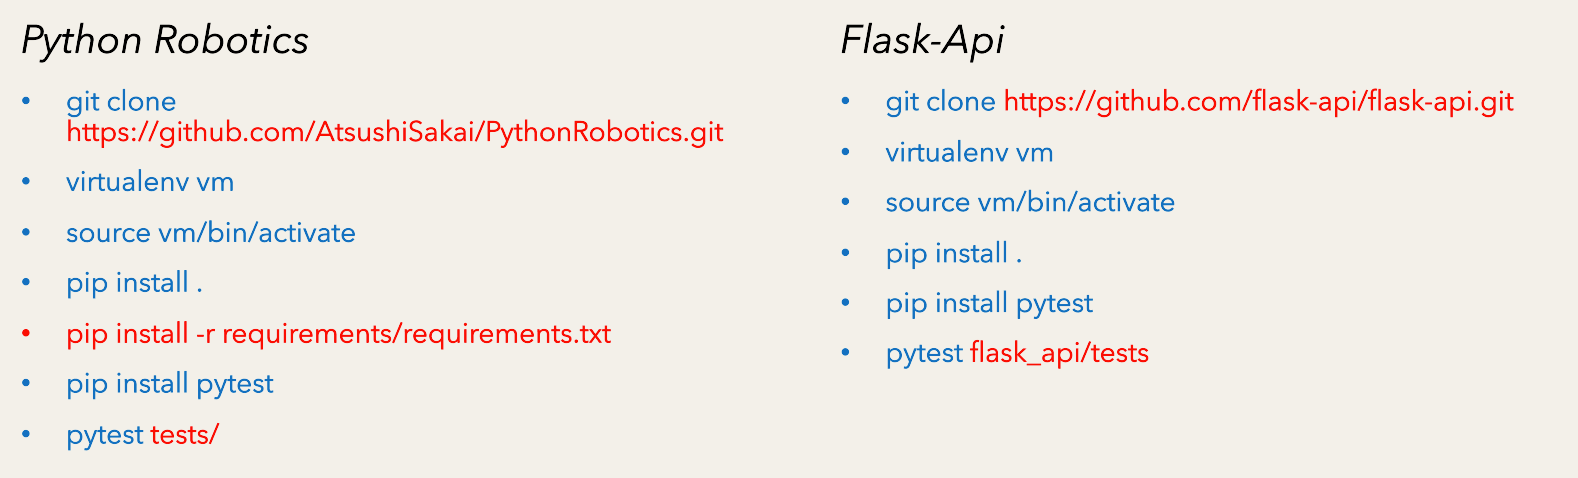
\includegraphics[width=1\linewidth]{figures/implementation/Setup-difference.png}
    \caption{Execution of Projects (Similarities and Differences)}
    \label{fig:setup difference}
\end{figure}

As can be seen from the Figure \ref{fig:setup difference}, the two commands of \textbf{git clone} and \textbf{pytest} have different argument values depending on the project.
To handle these difference we provide arguments to the bash script based on the project thereby making the automation generic.
These arguments are present in a text file, which is read by the bash script and the commands are run with the given arguments.
This text file is named as github-url.txt and contains a separate line for each project consisting of the GitHub URL and test directory path from the project root.
Furthermore, as can be seen from the Figure \ref{fig:setup difference}, Python Robotics project runs an extra command.
Execution of this command varies based on the presence or absence of the requirements file.
To handle this difference, github-url.txt file also contains a flag value for the project.
The flag value of \textit{rt} specifies the presence of requirements file, whereas the value \textit{t} indicates its absence.
We specify the path of the relevant requirements file for the project in case the flag value is \textit{rt}.
The Listing \ref{code:github-url-2} shows the entry of two projects shown in the Figure \ref{fig:setup difference}.

\lstset{numbers=left, numberstyle=\tiny, stepnumber=1, numbersep=5pt, columns=flexible, breaklines=true}
\lstset{basicstyle=\ttfamily}
\lstset{frame=tb}

\begin{lstlisting}[float,caption=Sample Entry github-url.txt,label=code:github-url-2,language=Bash]
https://github.com/AtsushiSakai/PythonRobotics.git rt requirements/requirements.txt tests
https://github.com/flask-api/flask-api.git t flask_api/tests
\end{lstlisting}

The bash script to automate the steps of installation of the 5 projects in section \ref{impl:first five} is shown in the Listing \ref{code:install-all-projects.sh}.
All the commands for installation shown in the Figure \ref{fig:setup difference} are present in this script.
We start by creating a common directory for all projects. 
Then we read the github-url.txt and loop over each line in the file indicated on line 20.
We split the line into parts to obtain the required argument for the concerned command.
Inside the folder created for each project, we clone the GitHub repository using the git clone command as shown on line 33.
After cloning the repository, we create the virtual environment and activate it as shown in lines 37 through 41.
Then the project is installed using pip as shown on the line 53.
This installs the project from the source code.
Next, on line 55 we check flag value for requirements file.
If present we install the dependencies from requirements file specified by its path on line 58.
On line 64, we install some dependencies for running the project test suite as these were missed during the installation.
We then finally install pytest library on line 68 and deactivate the virtual environment. 

\lstset{numbers=left, numberstyle=\tiny, stepnumber=1, numbersep=5pt, columns=flexible, breaklines=true, numberblanklines=false}
\lstset{basicstyle=\ttfamily}
\lstset{frame=tb}

\begin{lstlisting}[caption=Bash Script for Automation,label=code:install-all-projects.sh,language=Bash]
#root directory
ROOT_DIR=/DyPyBench
cd $ROOT_DIR

#read URL_FILE
URL_FILE=$ROOT_DIR/text/github-url.txt

# Create project folder to keep all the projects together inside one parent folder
PROJ_DIR=$ROOT_DIR/../Project
#if folder already present, then delete the folder
if [ -d "$PROJ_DIR" ]
then
    rm -rf "$PROJ_DIR" 
fi
mkdir -p "$PROJ_DIR"
cd "$PROJ_DIR"

#run a while loop for all projects
idx=1
while read line
do
    parts=($line)
    URL=${parts[0]}
    FLAGS=${parts[1]}
    
    #change to working directory
    cd $PROJ_DIR
    
    #create directory for project
    mkdir -p "project$idx"
    
    #clone the repo to project directory
    git clone "$URL" "project$idx"
    cd "project$idx"
    
    #create virtual env name .vm
    virtualenv .vm
    
    #activate virtual env
    if [[ -d ".vm/local" ]]
    then
        source .vm/local/bin/activate
    elif [[ -d ".vm/bin" ]]
    then
        source .vm/bin/activate
    else
        echo "Unable to create virtual env"
        exit
    fi

    #install using pip install . 
    echo "Running pip install ."
    pip install .

    if [[ $FLAGS == "rt" ]]
    then
        echo "Running pip install requirements"
        pip install -r $REQ_FILE
    fi

    #some projects need extra requirements for running test suites
    if [[ $URL == "https://github.com/lorien/grab.git" ]]
    then
        pip install cssselect pyquery pymongo fastrq #required for running tests
    fi

    #install pytest library
    pip install pytest

    ((idx++))
    deactivate

done < "$URL_FILE"
\end{lstlisting}

\section{Installing the Other 45 Projects}
\label{impl:size to 50}


\chapter{Evaluation}
\label{s:Evaluation}
In this chapter we discuss the experimental evaluation of DyPyBench. We do so by answering the following questions:

\textbf{RQ1:} How do the included test suites in Python projects within DyPyBench contribute to a dynamic benchmark?

\textbf{RQ2:} How efficient is our benchmark to generate (valid and good) training data for the neural models?

\textbf{RQ3:} How effective is DyPyBench to aid a comparison of static and dynamic call graph analysis?

Before answering the above questions, we detail the experimental setup for DyPyBench, neural model training and the call graph generation using static and dynamic analysis frameworks.
We further explain the evaluation criteria for measuring the effectiveness of DyPyBench.
% for the neural model and the analysis frameworks.
Finally, we discuss the evaluation and the results.

DyPyBench consists of 50 open-source python projects from different application domains list in Table \ref{table:50_installed_projects}.
We download the source code of these projects along with their test suite into a Docker image which contains the neural model (LExecutor) and the static (PyCG) and dynamic (DynaPyt) analysis frameworks.
We use these integrated test suites to execute the projects and collect various statistics and data.

\section{Experimental Setup for LExecutor}
We use DyPyBench to generate the training data for the neural model LExecutor.
LExecutor instruments the files and then generates traces from these files during run-time.
LExecutor provides its own instrumenter, and the accepts mandatory two arguments to perform instrumentation.
The first is a JSON file to store the mapping of iids and the second is files to instrument.
To generate the trace files, we execute the test suite consisting of the instrumented files.
The trace files from the above step are used to generate training data in the form of .pt files for the neural model.
For this task, LExecutor provides a module PrepareData which accepts the trace files and the JSON file created in the instrumentation step.
To generate the .pt file, LExecutor works in two modes of abstraction, fine-grained and coarse-grained.
At a time only one mode runs and this can be set in the Hyperparameters.py file.
The Listing \ref{code:Hyperparameters.py} shows the possible entries for the abstraction mode.
In this work, we generate the data using the two abstraction modes shown on line 1 and line 2 in the Listing \ref{code:Hyperparameters.py}. 
The PrepareData module also generates a validation file in the .pt format.
The trace entries are split into training and validation data based on the split provided in the Hyperparameters.py file as shown in Listing \ref{code:Hyperparameters.py} on line 3.
\begin{lstlisting}[caption=Abstraction Modes in LExecutor,label=code:Hyperparameters.py,language=Python]
    value_abstraction = "fine-grained"
    value_abstraction = "coarse-grained-deterministic"
    perc_train = 0.95
\end{lstlisting}

\section{Experimental Setup for PyCG}
PyCG generates call graph based on static analysis of code.
The call graphs is created in the JSON format, where the key is caller and the value is a list of called functions.
PyCG accepts 3 arguments, the package contains the source files, the entry point files and the output file save the JSON.
In DyPyBench, we provide the package as source code cloned from Git and the test files as entry point files for each project.
The execution of the PyCG module then provides us with the call graph in the mentioned JSON format.

\section{Experimental Setup for DynaPyt}
DynaPyt instruments the files and the execution of the instrumented code provides us with the dynamic analysis.
DynaPyt, has its own modules for instrumentation and analysis.
We first use the instrumentation module to instrument the source files.
To run the analysis, we create a entry file to run all the test files using the main function provided by the pytest module.
Additionally, we provide the option of import-mode set to importlib to the pytest.main function.
We add the Call Graph analysis is DynaPyt with the function pre\_call hook, and specify this analysis to the analysis module of DynaPyt.
The analysis generates the output in the JSON format, with the key as caller and the value as a list of called functions.
The JSON is stored in a file at the end of the execution of the analysis.
Listing \ref{code:CallGraphAnalysis} provides the code for the analysis written in DynaPyt.

\section{Evaluation Criteria}
We use different evaluation criteria for each of the three questions mentioned above.
First, the criteria to measure the dynamic nature of DyPyBench is the statistics of executing test suites.
These include the number of passed and failed test cases and also the running time of the test suites.
Second, for measuring the effectiveness of DyPyBench for neural model the criteria is the number of data points we collect and the accuracy of the model.
The number of data point refers to the number of unique use-value events used by LExecutor to train and validate the neural model.
The accuracy of the model refers to the how correctly can the model predict the missing input value to execute the arbitrary code using LExecutor. 
Lastly, the criteria for measuring the effectiveness for analysis frameworks is the statistics of static and dynamic call graph comparisons.
The statistics include the imprecision and number of matching and non-matching callers and callees.
The imprecision occurs when one callee in DynaPyt matches to two or more callees in PyCG, due the implementation differences of the two frameworks.

\section{Results}

\subsection{Effectiveness of Test Suite}
Addressing \textbf{RQ1}, we find that DyPyBench provides 45086 test cases and the running time of test suites is between 0.02 seconds and 1362.86 seconds.
Overall, 41451 test cases pass where as 429 fail.
The successful execution of such a high number of test cases makes our benchmark dynamic in nature.
The number of projects which have 0 failed test cases in DyPyBench is 31, whereas 13 others have failed tests between 1 and 10.
The number of test cases in each project varies from 1 to 10552.
Figure \ref{fig:successful_tests} shows the percentage of passed test cases in all projects of DyPyBench.
We see that 41 projects have more than 90\% passed test cases, while 46 have 80\% or more passed test cases.
\begin{figure}[ht]
    \centering
    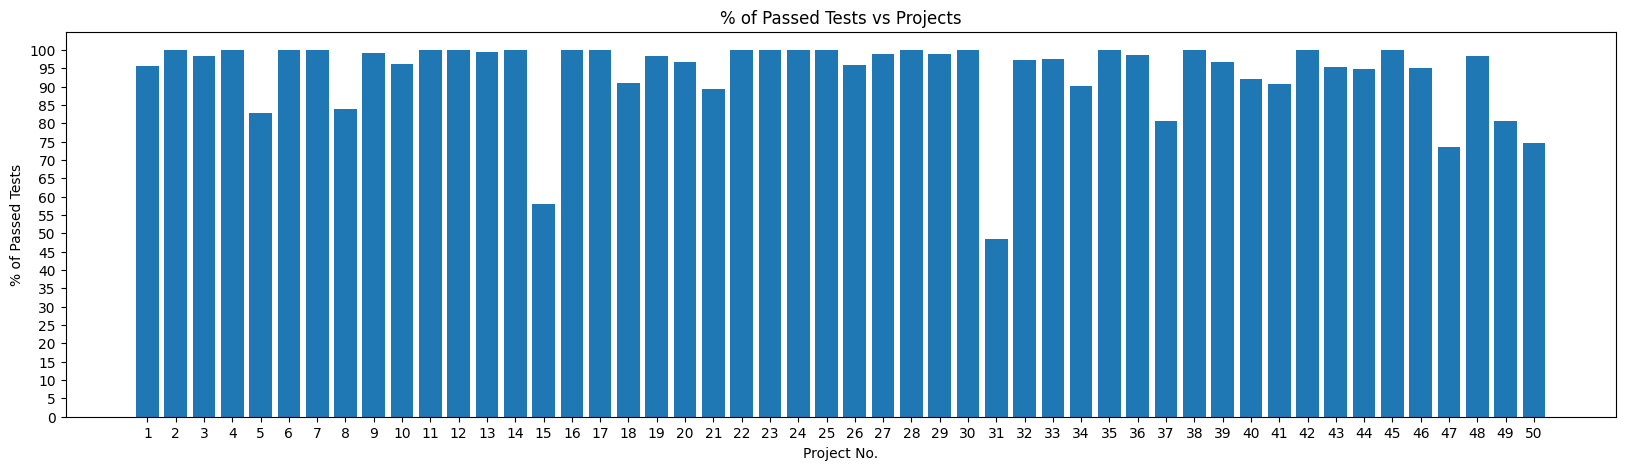
\includegraphics[width=1\linewidth]{figures/evaluation/perc_passed_tests.png}
    \caption[Passed Test Case Percentage]{\label{fig:successful_tests}Percentage of Passed Tests in DyPyBench Projects}
\end{figure}

Since the execution of the project is important for dynamic analysis, the high pass percentage of 91.93\% for all tests cases is an advantage for efficient analysis.
The running time for each project is shown in Table \ref{fig:test_run_times}.
The total run time for all the projects in DyPyBench is 3568.86 seconds.
There are 39 projects which run the test suite within 50 seconds.
\begin{figure}[ht]
    \centering
    % 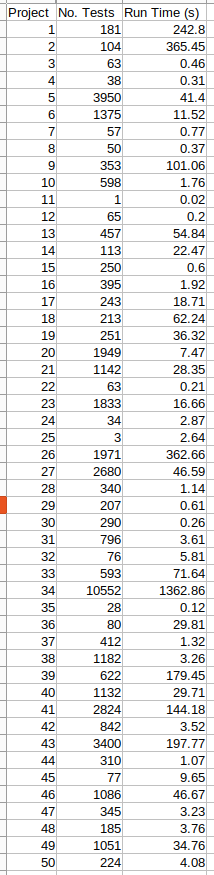
\includegraphics[width=0.4\linewidth,height=1.3\linewidth]{figures/evaluation/test_runtime.png}
    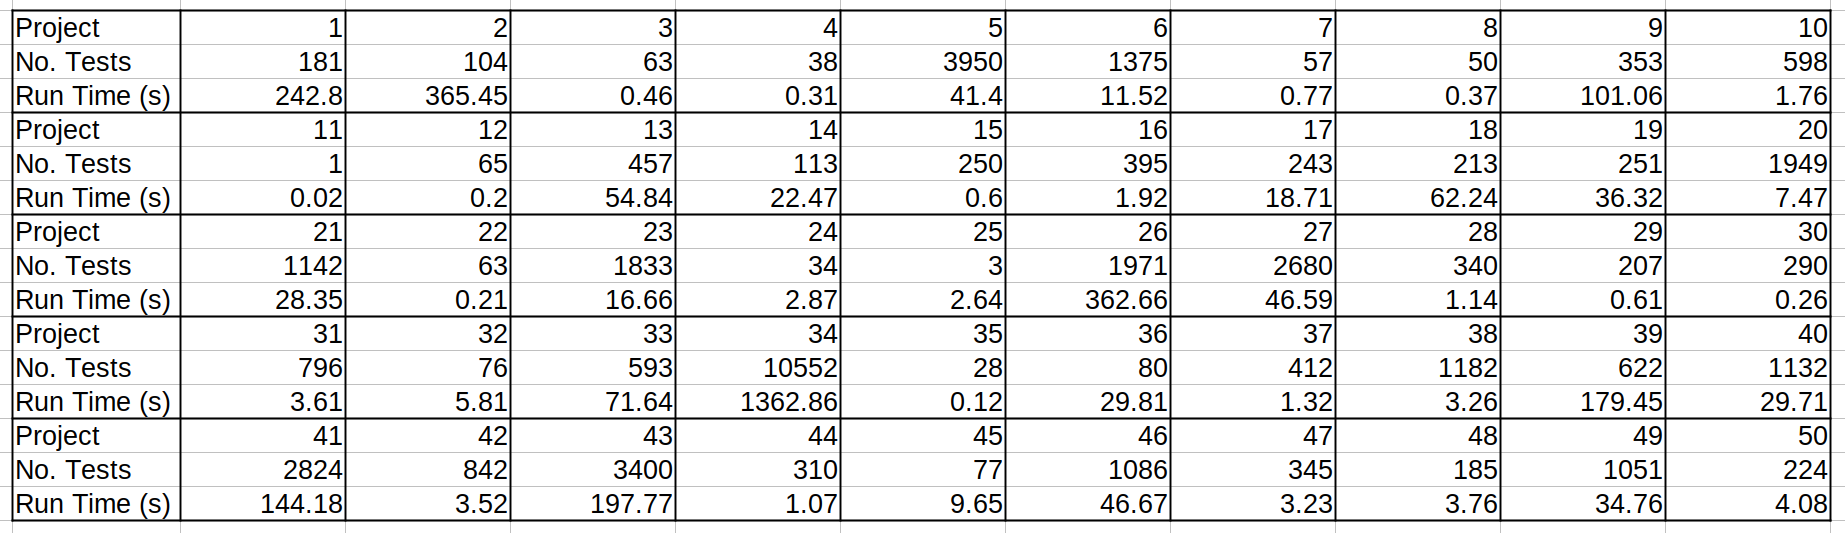
\includegraphics[width=1\linewidth]{figures/evaluation/tests_runtime2.png}
    \caption[Test Suite Run Time]{\label{fig:test_run_times}Test Suite Run Time in DyPyBench Projects}
\end{figure}

\subsection{Effectiveness for Neural Model}
Addressing \textbf{RQ2}, we find that DyPyBench contributes 547,830 new data points. 
This results in the model accuracy between 71.86\% and 93.67\% after training the model.

The new data points we found are generated from 37 projects in our benchmark and amount to nearly 2.5 times the data points used by LExecutor.
The Figure \ref{fig:Lex_projects_events} shows the data points from each project labelled with project number.
As can be seen from the Figure \ref{fig:Lex_projects_events}, the distribution of these data points vary from project to project.
This can be attributed to the number of files in each project that are instrumented. 
\begin{figure}[ht]
    \centering
    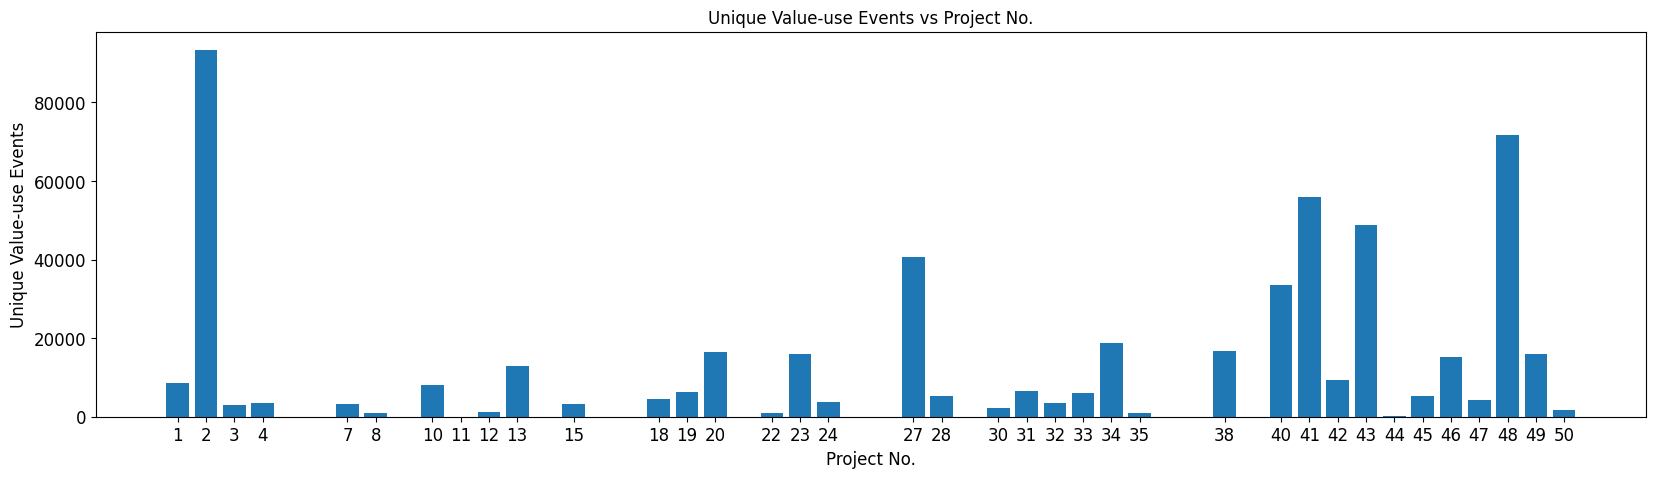
\includegraphics[width=1\linewidth]{figures/evaluation/lex_data_points.png}
    \caption[Unique Value-use Events]{\label{fig:Lex_projects_events}Unique Value-use Events in DyPyBench Projects}
\end{figure}

To evaluate the accuracy of the neural model based on the new data points, we perform a total of 6 experiments using different validation data and the abstraction modes.
Overall, we use 3 different validation data-sets.
First is a random split of 5\% from the data points we found with 37 projects in DyPyBench, second is the data-set provided by the LExecutor. This data-set has data points which were not for training the model.
Finally, the third data-set is the split from the new data points by projects. 6 projects were selected at random, which constitute nearly 5\% of the data points and these projects were excluded from 
training data-set.
For each of the validation data-set we perform 2 experiments, one with the abstraction mode as fine-grained while the other with coarse-grained as described before.

\begin{figure}[ht]
    \centering
    \subfigure[Fine-grained]{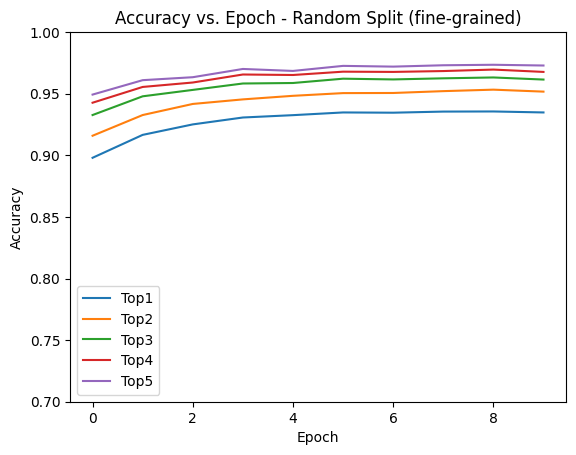
\includegraphics[width=0.4\linewidth]{figures/evaluation/lex_random_fine.png}}
    \subfigure[Coarse-grained]{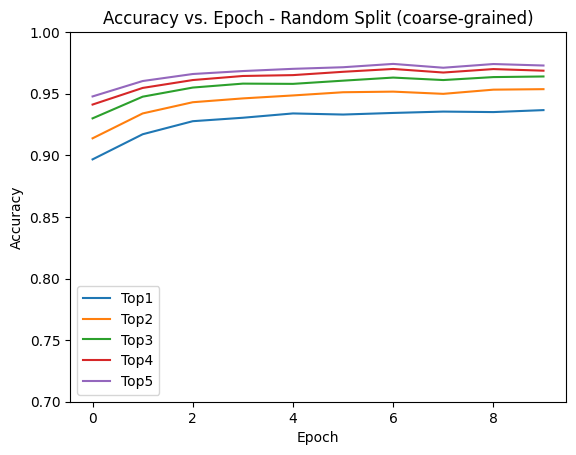
\includegraphics[width=0.4\linewidth]{figures/evaluation/lex_random_coarse.png}}
    \caption[Accuracy vs Epoch (Random Split)]{\label{fig:lex_random}Accuracy vs Epoch (Random Split) }
\end{figure}

Figure \ref{fig:lex_random} shows how the accuracy of the model varies with the number of epochs when the first validation data-set mentioned above is used.
Each line in the Figure \ref{fig:lex_random} shows the accuracy for top-n predictions for the same input.
As can be seen, the accuracy for top-5 is the best followed by top-4 and so on.
We mainly consider the accuracy of the first prediction, which starts at nearly 90\% and improves up to 93\% for both fine and coarse grained.

\begin{figure}[ht]
    \centering
    \subfigure[Fine-grained]{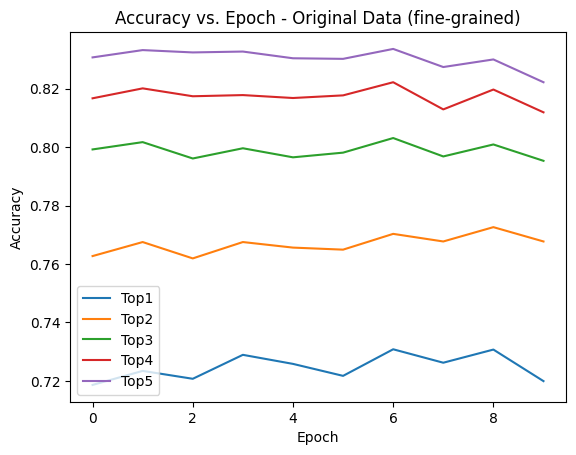
\includegraphics[width=0.4\linewidth]{figures/evaluation/lex_original_fine.png}}
    \subfigure[Coarse-grained]{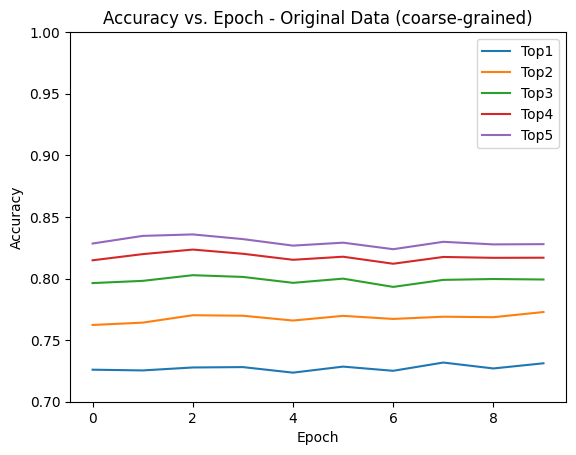
\includegraphics[width=0.4\linewidth]{figures/evaluation/lex_original_coarse.png}}
    \caption[Accuracy vs Epoch (Original Data)]{\label{fig:lex_original}Accuracy vs Epoch (Original Data) }
\end{figure}

Similarly, Figure \ref{fig:lex_original} shows the accuracy versus epoch for validation data-set used by the LExecutor.
As we can see in the Figure \ref{fig:lex_original}, the accuracy is lower than the previous experiments plunging down to 73\% in both cases of abstraction.
Finally, the Figure \ref{fig:lex_project} shows the accuracy versus epoch comparison for the third validation data-set mentioned above.
In this case, the accuracy ranges between the previous two experiments having the value of 85\% for both levels of abstraction.
For the first and second validation data-set, we get the best model in the 7th and 8th epoch.
However, for the third data-set the best model is found at the 4th epoch itself.
Since, the neural model we start with is a pre-trained model, the accuracy range we found is similar to the one specified by LExecutor.

\begin{figure}[ht]
    \centering
    \subfigure[Fine-grained]{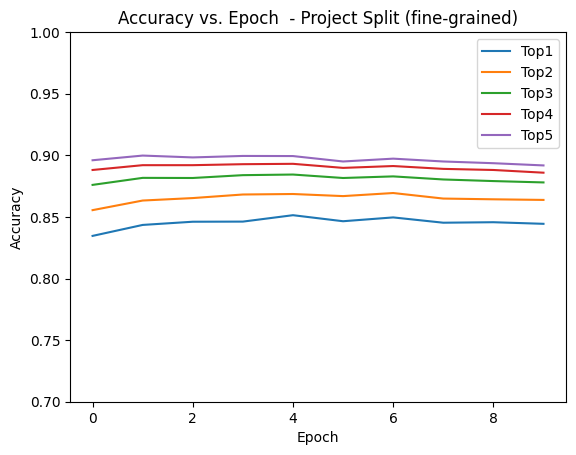
\includegraphics[width=0.4\linewidth]{figures/evaluation/lex_project_fine.png}}
    \subfigure[Coarse-grained]{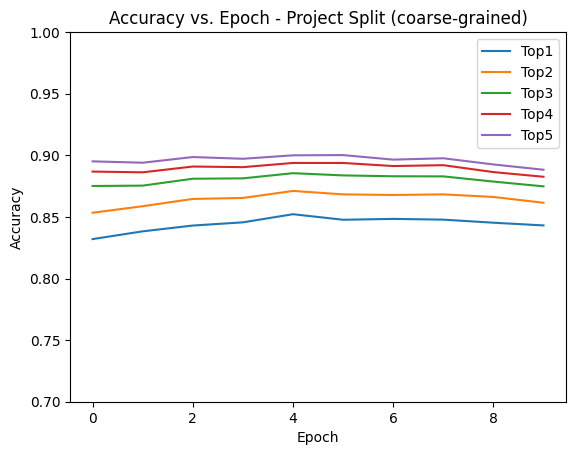
\includegraphics[width=0.4\linewidth]{figures/evaluation/lex_project_coarse.png}}
    \caption[Accuracy vs Epoch (Project Split)]{\label{fig:lex_project}Accuracy vs Epoch (Project Split) }
\end{figure}


\subsection{Effectiveness for Analysis Frameworks}
Addressing \textbf{RQ3}, we find that 

\chapter{Related Work}
\label{s:Related Work}
In this chapter, we outline some of the work done on benchmarks.
We also discuss some of the work done on dynamic analysis.

\section{Benchmarks}
% In the context of software development, a benchmark is a standardized set of tests that are designed to measure the performance of a system or application.
% These tests are typically used to assess the speed, scalability, and resource utilization of a given system, and can be an important tool for developers seeking to optimize their code and improve overall performance.
% When it comes to evaluating the performance of a software system, there are two primary types of benchmarks: static benchmarks and dynamic benchmarks.
% Static benchmarks involve running a predetermined set of tests on a given system or application, with fixed input parameters and test conditions. These benchmarks are useful for measuring the absolute performance of a system under a specific set of circumstances, and can be used to compare the performance of different systems or implementations against one another.
% Dynamic benchmarks involve running a set of tests that are designed to adapt and respond to the behavior of the system being tested. These benchmarks are typically more complex than static benchmarks, and are designed to simulate real-world usage scenarios and workloads.
% One of the main benefits of dynamic benchmarks is that they provide a more accurate and realistic assessment of system performance than static benchmarks.
% Because dynamic benchmarks can adapt to the behavior of the system being tested, they can capture a wider range of use cases and performance characteristics that may not be captured by static benchmarks alone.

% \textit{DaCapo Benchmark.} Traditional benchmarks, such as those developed for C, C++, and Fortran, typically focus on static properties, such as code complexity and code size.
% However, there is a need for benchmarks that can account for dynamic properties, such as memory management and garbage collection.
Dynamic benchmarks, such as the DaCapo benchmark suite, provide a more comprehensive evaluation of software systems by taking into account the interactions between architecture, compiler, virtual machine, memory management, and application. These benchmarks evaluate the performance of software systems under more realistic conditions, allowing researchers and developers to better understand how their systems will perform in the real world. \cite{DaCapo_2006}
The SPEC C++ benchmarks, including SPEC CPU2006 C++, SPEC OMP2012, and SPEC MPI2007 are designed to evaluate the performance of C++ compilers, libraries, and hardware platforms. These benchmarks are valuable for developers and researchers seeking to optimize the performance of C++ programs, as they provide insights into the performance characteristics of their code and can be used to compare the performance of different C++ compilers and libraries on different hardware platforms. \cite{SPEC_C++_2006, SPEC_OMP_2012, SPEC_MPI_2007}
While, DaCapo and SPEC C++ Benchmark provide a dynamic benchmark for Java and C++, Python does not have one. DyPyBench, overcomes this ba providing a dynamic benchmark for Python.    

\section{Dynamic Analysis}
The analysis of properties of a running program is known as dynamic analysis.\cite{Ball_1999}
Dynamic analysis can be particularly useful in complex software systems, where issues may be difficult to identify or diagnose through manual testing alone.
\cite{dynamic_analysis}
TaintCheck proposes dynamic taint analysis for automatic detection and analysis of software vulnerabilities. The approach is to performs binary rewriting at run time and reliably detects most types of exploits without false positives.\cite{newsome2005dynamic}
Branch Coverage analysis counts program branch execution and outcome frequency with a single API hook. Results are stored in a dictionary mapping branch location and condition value to event occurrences. The hierarchy captures all branching events, enabling effective analysis with minimal implementation.\cite{DynaPyt2022}
DyPyBench provides a call graph analysis to generate call graphs during run-time for Python programs. 
% The first experimental study on dynamic opcode analysis of cryptomining has shown that browser-based cryptomining can be detected with accuracies up to 100\%, offering an opportunity to rapidly detect, prevent, and mitigate such attacks.\cite{Dynamic_analysis_usage}

% Dynamic analysis is a software testing technique that involves evaluating the behavior of a running program or system in real-time.
% Unlike static analysis, which involves analyzing the source code of a program without actually running it, dynamic analysis involves monitoring the behavior of a program as it runs, to identify bugs, errors, and other issues that may not be apparent from the source code alone.
% One of the primary benefits of dynamic analysis is that it allows developers to identify and diagnose issues that may be difficult or impossible to detect through static analysis alone.
% For example, dynamic analysis can be used to identify memory leaks, race conditions, and other types of concurrency issues that may not be apparent from the source code alone.
% Dynamic analysis can be particularly useful in complex software systems, where issues may be difficult to identify or diagnose through manual testing alone.
% \cite{dynamic_analysis}

% \textit{DynaPyt Framework.} DynaPyt is the first general-purpose framework for heavy-weight dynamic analysis of Python programs. DynaPyt offers a wider range of analysis hooks and features selective instrumentation and execution modification. The framework is evaluated on 9 open-source Python projects totaling 1,268,545 lines of code and shows that it preserves the semantics of the original execution. DynaPyt's running time is in line with similar frameworks designed for other languages and is faster than analyses using Python's built-in tracing API. Several analyses are implemented, including detecting memory blow-ups, taint analysis for SQL injections, and warning about runtime performance anti-patterns. Implementation of new analyses for potential use cases is simple in DynaPyt. DynaPyt provides a valuable tool for developers and researchers seeking to optimize the performance and security of Python programs through dynamic analysis. \cite{DynaPyt2022}

% While DynaPyt provides us some sample analyses, DyPyBench adds a new one to its arsenal and uses it on a number of projects. This analyses is named as Call Graph and it generates run-time call graphs for the projects in DyPyBench. 

% \section{Neural Networks for Input Prediction}
% Neural networks for code prediction involve training models to predict the input that a software program requires based on contextual information, such as user behavior, previous inputs, or external events.
% These models have potential applications in automating programming tasks and facilitating collaboration between developers with varying levels of expertise.

% \textit{LExecutor.} Executing code is important for various program analysis tasks, but it can be difficult due to missing definitions, inputs, and dependencies. LExecutor is a learning-guided approach for executing arbitrary code snippets by letting a neural model predict missing values and injecting them into the execution. For instance, LExecutor injects likely values for undefined variables and likely return values of missing functions. The approach is evaluated on Python code from popular open-source projects and code snippets from Stack Overflow. The neural model predicts realistic values with an accuracy between 80.1\% and 94.2\%, allowing LExecutor to closely mimic real executions. As a result, LExecutor successfully executes significantly more code than other techniques, covering 50.1\% of all lines compared to 4.1\% when executing the code as-is. LExecutor provides a promising approach for executing underconstrained code snippets, enabling more comprehensive and accurate program analysis. \cite{LExecutor_2023}

% With more data, the neural model can learn more complex patterns and relationships, leading to a better understanding of the underlying data distribution. DyPyBench provides this extra data for LExecutor to generalize and improve the accuracy of the model.

\chapter{Conclusion}
\label{s:Conclusion}
% This work highlights the importance of dynamic benchmarks and identifies the lack of such benchmarks in Python.
To address this gap, we present DyPyBench, a dynamic benchmark comprising 50 diverse and readily usable projects.
Our benchmark is ready-to-run, extensible, and ready-to-analyze for researchers and developers.

To evaluate the effectiveness of DyPyBench, we use various tools such as LExecutor, DynaPyt, and PyCG.
Our benchmark provides 41,451 successful test cases, which generate 547,830 data points for LExecutor.
The accuracy of the neural model for predicting input values to execute arbitrary code snippets ranges between 71.86\% and 93.67\%.
Additionally, DyPyBench generates data points for comparing static and dynamic call graph analysis using DynaPyt and PyCG.
We achieve matching percentages of 51.93\% and 66.41\% for callers and 47.58\% and 28.58\% for callees in PyCG and DynaPyt, respectively.

The key insight of our is that DyPyBench is a versatile benchmark framework that can be used with various code analysis tools.
By providing a readily available Docker image with integrated analysis tools, we make it easier for researchers and developers to use DyPyBench.

We envision DyPyBench as a benchmark framework for dynamic analysis of Python projects that can generate valuable data to aid research in code analysis tasks.

\appendix
\chapter{Awesome Python Projects}
\label{appendix:awesome python projects}

% \section{Awesome Python Project}
% \label{appendix:awesome python projects}
\begin{table}[ht]
    \centering
    \begin{tabular}{|l|c|}
    \hline
    \textbf{Category} & \textbf{Number of Projects}\\
    \hline
    Admin Panels & 9\\
    Algorithms and Design Patterns & \\
    Algorithms & 4\\
    Design Patterns & 3\\
    ASGI Servers & 2\\
    Asynchronous Programming & 2\\
    Audio & \\
    Audio & 9\\
    Metadata & 4\\
    Authentication & \\
    OAuth & 7\\
    JWT & 3\\
    Build Tools & 5\\
    Built-in Class Enhancement & 5\\
    CMS & 8\\
    Caching & 7\\
    ChatOps Tools & 1\\
    Code Analysis & \\
    Code Analysis & 5\\
    Code Linters & 4\\
    Code Formatters & 3\\
    Static Type Checkers & 3\\
    Static Type Annotation Generators & 3\\
    Command Line Interface Development & \\
    Command Line Application Development & 6\\
    Terminal Rendering & 6\\
    Command Line Tools & \\
    Productivity tools & 10\\
    CLI Enhancement & 7\\
    Compatibility & 3\\
    Computer Vision & 7\\
    Concurrency and Parallelism & 6\\
    Configuration & 5\\
    Cryptography & 4\\
    Data Analysis & 6\\
    Data Validation & 7\\
    Data Visualization & 13\\
    Database & 3\\
    Database Drivers & \\
    MySQL & 2\\
    PostgreSQL  & 2\\
    SQlite & 2\\
    Other Relational databases & 2\\
    NoSQL databases & 6\\
    Asynchronous Clients & 1\\
    Date and Time & 10\\
    \end{tabular}
    \caption{Awesome Python Project Categories and Numbers}
\end{table}

\begin{table}[ht]
\centering
\begin{tabular}{|l|c|}
\hline
\textbf{Category} & \textbf{Number of Projects}\\
\hline
Debugging Tools & \\
pdb-like debugger & 4\\
tracing & 4\\
profiler & 5\\
others & 5\\
Deep Learning & 7\\
DevOps Tools & \\
configuration management & 5\\
ssh style deployment & 3\\
process management & 2\\
monitoring & 1\\
backup & 1\\
others & 1\\
Distributed Computing & \\
batch processing & 5\\
stream processing & 2\\
Distribution & 8\\
Documentation & 3\\
Downloader & 5\\
E-Commerce & 10\\
Editor plugins and IDE & \\
Emacs & 1\\
Sublime & 2\\
Vim & 3\\
Visual Studio & 1\\
VS Code & 1\\
IDE & 2\\
Email & \\
mail servers & 2\\
clients & 2\\
others & 2\\
Enterprise Application Integration & 1\\
Environment Management & 2\\
Files & 7\\
Foreign Function Interface & 4\\
Forms & 6\\
Functional Programming & 7\\
GUI Development & 16\\
GraphQL & 4\\
Game Development & 9\\
Geolocation & 5\\
HTML Manipulation & 11\\
HTTP Clients & 6\\
Hardware & 7\\
Image Processing & 15\\
\hline
\end{tabular}
\caption[Awesome Python]{\label{table:awesome-python2}Awesome Python.}
\end{table}

\begin{table}[ht]
\centering
\begin{tabular}{ll}
\hline
\textbf{Category} & \textbf{Number of Projects}\\
\hline
Implementations & 13\\
Interactive Interpreter & 3\\
Internationalization & 2\\
Job Scheduler & 11\\
Logging & 5\\
Machine Learning & 9\\
Microsoft Windows & 5\\
Miscellaneous & 6\\
Natural Language Processing & \\
general & 9\\
chinese & 4\\
Network Virtualization & 3\\
News Feed & 2\\
ORM & \\
relational databases & 8\\
noSQL databases & 4\\
Package Management & 3\\
Package Repositories & 4\\
Penetration Testing & 3\\
Permissions & 2\\
Processes & 3\\
Recommender Systems & 8\\
Refactoring & 3\\
RESTful API & \\
Django & 2\\
Flask & 3\\
Pyramid & 1\\
Framework agnositic & 7\\
Robotics & 2\\
RPC Servers & 2\\
Science & 21\\
Search & 5\\
Serialization & 4\\
Serverless Frameworks & 2\\
Shell & 1\\
Specific Formats processing & \\
general & 1\\
office & 9\\
pdf & 3\\
markdown & 2\\
yaml & 1\\
csv & 1\\
archive & 1\\
\hline
\end{tabular}
\caption[Awesome Python]{\label{table:awesome-python3}Awesome Python.}
\end{table}

\begin{table}[ht]
\centering
\begin{tabular}{ll}
\hline
\textbf{Category} & \textbf{Number of Projects}\\
\hline
Static Site Generator & 5\\
Tagging & 1\\
Task Queues & 5\\
Template Engine & 3\\
Testing & \\
testing frameworks & 5\\
test runners & 3\\
GUI / Web testing & 6\\
Mock & 8\\
Object Factories & 3\\
Code Coverage & 1\\
Fake data & 4\\
Text Processing & \\
general & 10\\
slugify & 3\\
unique indentifiers & 2\\
parser & 7\\
Third Party API’s & 7\\
URL Manipulation & 4\\
Video & 3\\
Web Asset Management & 7\\
Web Content Extracting & 9\\
Web Crawling & 8\\
Web Frameworks & \\
synchronous & 4\\
asynchronous & 1\\
Web Sockets & 3\\
WSGI Servers & 5\\
\hline
\end{tabular}
\caption[Awesome Python]{\label{table:awesome-python4}Awesome Python.}
\end{table}


% \chapter{Great Work}
% \label{s:GreatWork}

% This and the following chapters detail the original work.

% \chapter{Examples}
% \label{s:Examples}

% This chapter provides some additional hints and examples for the
% layout and style of the thesis. It is worthwhile to look at the source
% file \verb|Examples.tex| for this appendix to understand how it was
% created.

% \section{Tables}

% Tables are left justified and the caption appears on top as seen in
% Table~\ref{t:Translations}.

% \begin{table}[ht]
% \centering
% \begin{tabular}{ll}
% \hline
% \textbf{English} & \textbf{German}\\
% \hline
% cell phone       & Handy\\
% Diet Coke        & Coca Cola light\\
% \hline
% \end{tabular}
% \caption[Translations]{\label{t:Translations}Translations.}
% \end{table}

% \section{Figures}

% Figure~\ref{f:SOLAlogo} shows a simple figure with a single picture
% and Figure~\ref{f:SubfigureExample} shows a more complex figure
% containing subfigures.

% \begin{figure}[ht]
% \centering
% 
\includegraphics[width=.6\linewidth]{figures/SOLALogo}
% \caption[SOLA logo]{\label{f:SOLAlogo}SOLA logo.}
% \end{figure}

% \begin{figure}[ht]
% \centering
% \subfigure[UStuttLogo]{
\includegraphics[height=12mm]{figures/UStuttLogo}}\quad
% \subfigure[SOLALogo]{
\includegraphics[height=12mm]{figures/SOLALogo}}
% \caption[Subfigure example]{\label{f:SubfigureExample}Two pictures as
%   part of a single figure through the magic of the subfigure package.}
% \end{figure}

% \section{Units}

% The SIUnits package provides nice spacing for units as demonstrated in
% Table~\ref{t:SIUnits}. Use of the package also makes it easy to change
% the style or even the unit text in the future.

% \begin{table}[ht]
% \centering
% \begin{tabular}{ll}
% \hline
% \textbf{Output}   & \textbf{Command}\\
% \hline
% 42m               & \verb|42m|\\
% \unit{42}{\metre} & \verb|\unit{42}{\metre}|\\
% 42 m              & \verb|42 m|\\
% \hline
% \end{tabular}
% \caption[Spacing for units]{\label{t:SIUnits}Spacing for units.}
% \end{table}

% \section{Source code}

% The listings package provides tools to typeset source code
% listings. It supports many programming languages and provides a lot of
% formatting options.

% \lstset{numbers=left, numberstyle=\tiny, stepnumber=1, numbersep=5pt}
% \lstset{basicstyle=\ttfamily}
% \lstset{frame=tb}

% \begin{lstlisting}[float,caption=Example usage of the listing package,label=l:javaClass,language=Java]
% class S {
%    int f1 = 42;
%    public S(int x) {
%           f1 = x;
%    }
% }
% \end{lstlisting}

% Listing \ref{l:javaClass} shows an example listing. Code snippets can
% also be inserted in normal text:
% \verb$\lstinline|int f1 = 42;|$ gives \lstinline$int f1 = 42;$

% \section{Miscellany}

% \begin{description}

% \item[Capitalization.] When referring to a named table (such as in the
%   previous section), the word \emph{table} is capitalized. The same is
%   true for figures, chapters and sections.

% \item[Bibliography.] Use \verb|bibtex| to make your life easier and to
%   produce consistently formatted entries.

% \item[Contractions.] Avoid contractions. For instance, use ``do not''
%   rather than ``don't.''

% \item[Style guide.] A classic reference book on writing style is
%   Strunk's \emph{The Elements of Style} \cite{Strunk-ElementsOfStyle}.

% \end{description}

% % -------------------------------------------------------------------------------------------------
% % Appendices (if needed)
% % -------------------------------------------------------------------------------------------------
% \appendix
% \chapter{Extra Stuff}
% \label{s:ExtraStuff}

% Additional material such as long mathematical derivations.

% -------------------------------------------------------------------------------------------------
% Bibliography
% -------------------------------------------------------------------------------------------------
\addcontentsline{toc}{chapter}{Bibliography}
\bibliography{report}

\chapter*{}

\vspace{-14em}
\textbf{Selbsst\"andigkeitserkl\"arung}\\

\noindent

Ich versichere, diese Arbeit selbstst\"andig verfasst zu haben. Ich habe keine anderen als die
angegebenen Quellen benutzt und alle w\"ortlich oder sinngem\"a{\ss} aus anderen Werken \"ubernommenen
Aussagen als solche gekennzeichnet. Weder diese Arbeit noch wesentliche Teile daraus waren bisher
Gegenstand eines anderen Pr\"ufungsverfahrens. Ich habe diese Arbeit bisher weder teilweise noch
vollst\"andig ver\"offentlicht.
Das elektronische Exemplar stimmt mit allen eingereichten Exemplaren \"uberein.

\vspace{8em}
\noindent\begin{tabular}{p{0.5\linewidth}p{0.4\linewidth}}
\rule{0.25\textwidth}{0.4pt} & \rule{0.4\textwidth}{0.4pt} \\
\textbf{Datum} & \textbf{Unterschrift}  \\
\end{tabular}


\end{document}
